\documentclass{article}
\usepackage[utf8x]{inputenc}
\usepackage{ucs}
\usepackage{amsmath} 
\usepackage{mathtext}
\usepackage{amsfonts}
\usepackage{upgreek}
\usepackage[english,russian]{babel}
\usepackage{graphicx}
\usepackage{float}
\usepackage{textcomp}
\usepackage{hyperref}
\usepackage{geometry}
  \geometry{left=2cm}
  \geometry{right=1.5cm}
  \geometry{top=1cm}
  \geometry{bottom=2cm}
\usepackage{tikz}
\usepackage{ccaption}
\usepackage{multicol}

\usepackage{listings}
%\setlength{\columnsep}{1.5cm}
%\setlength{\columnseprule}{0.2pt}


\begin{document}
\pagenumbering{gobble}

\lstset{
  language=C,                % choose the language of the code
  basicstyle=\linespread{1.1}\ttfamily,
  columns=fixed,
  fontadjust=true,
  basewidth=0.5em,
  keywordstyle=\color{blue}\bfseries,
  commentstyle=\color{gray},
  stringstyle=\ttfamily\color{orange!50!black},
  showstringspaces=false,
  %numbers=false,                   % where to put the line-numbers
  numbersep=5pt,
  numberstyle=\tiny\color{black},
  numberfirstline=true,
  stepnumber=1,                   % the step between two line-numbers.        
  numbersep=10pt,                  % how far the line-numbers are from the code
  backgroundcolor=\color{white},  % choose the background color. You must add \usepackage{color}
  showstringspaces=false,         % underline spaces within strings
  captionpos=b,                   % sets the caption-position to bottom
  breaklines=true,                % sets automatic line breaking
  breakatwhitespace=true,         % sets if automatic breaks should only happen at whitespace
  xleftmargin=.2in,
  extendedchars=\true,
  keepspaces = true,
}
\lstset{literate=%
   *{0}{{{\color{red!20!violet}0}}}1
    {1}{{{\color{red!20!violet}1}}}1
    {2}{{{\color{red!20!violet}2}}}1
    {3}{{{\color{red!20!violet}3}}}1
    {4}{{{\color{red!20!violet}4}}}1
    {5}{{{\color{red!20!violet}5}}}1
    {6}{{{\color{red!20!violet}6}}}1
    {7}{{{\color{red!20!violet}7}}}1
    {8}{{{\color{red!20!violet}8}}}1
    {9}{{{\color{red!20!violet}9}}}1
}


\section*{Задачи:}
\begin{multicols}{2}
\begin{lstlisting}
// Шаблоны
template <class T>
T GetMax (T a, T b) {
  T result;
  result = (a>b)? a : b;
  return (result);
}
int main () 
{
  int i=5, j=6, k;
  long l=10, m=5, n;
  k=GetMax<int>(i,j);
  n=GetMax<long>(l,m);
}

// Векторы
  std::vector<int> myvector;
  for (int i=1; i<=5; i++) myvector.push_back(i);

  for (std::vector<int>::iterator it = myvector.begin() ; it != myvector.end(); ++it)
    std::cout << ' ' << *it;




// Множества
  std::set<int> myset;
  std::set<int>::iterator it;

  // set some initial values:
  for (int i=1; i<=5; i++) myset.insert(i*10);    // set: 10 20 30 40 50

  it=myset.find(20);
  myset.erase (it);
  myset.erase (myset.find(40));

  std::cout << "myset contains:";
  for (it=myset.begin(); it!=myset.end(); ++it)
    std::cout << ' ' << *it;
  std::cout << '\n';
\end{lstlisting}
\begin{center}
%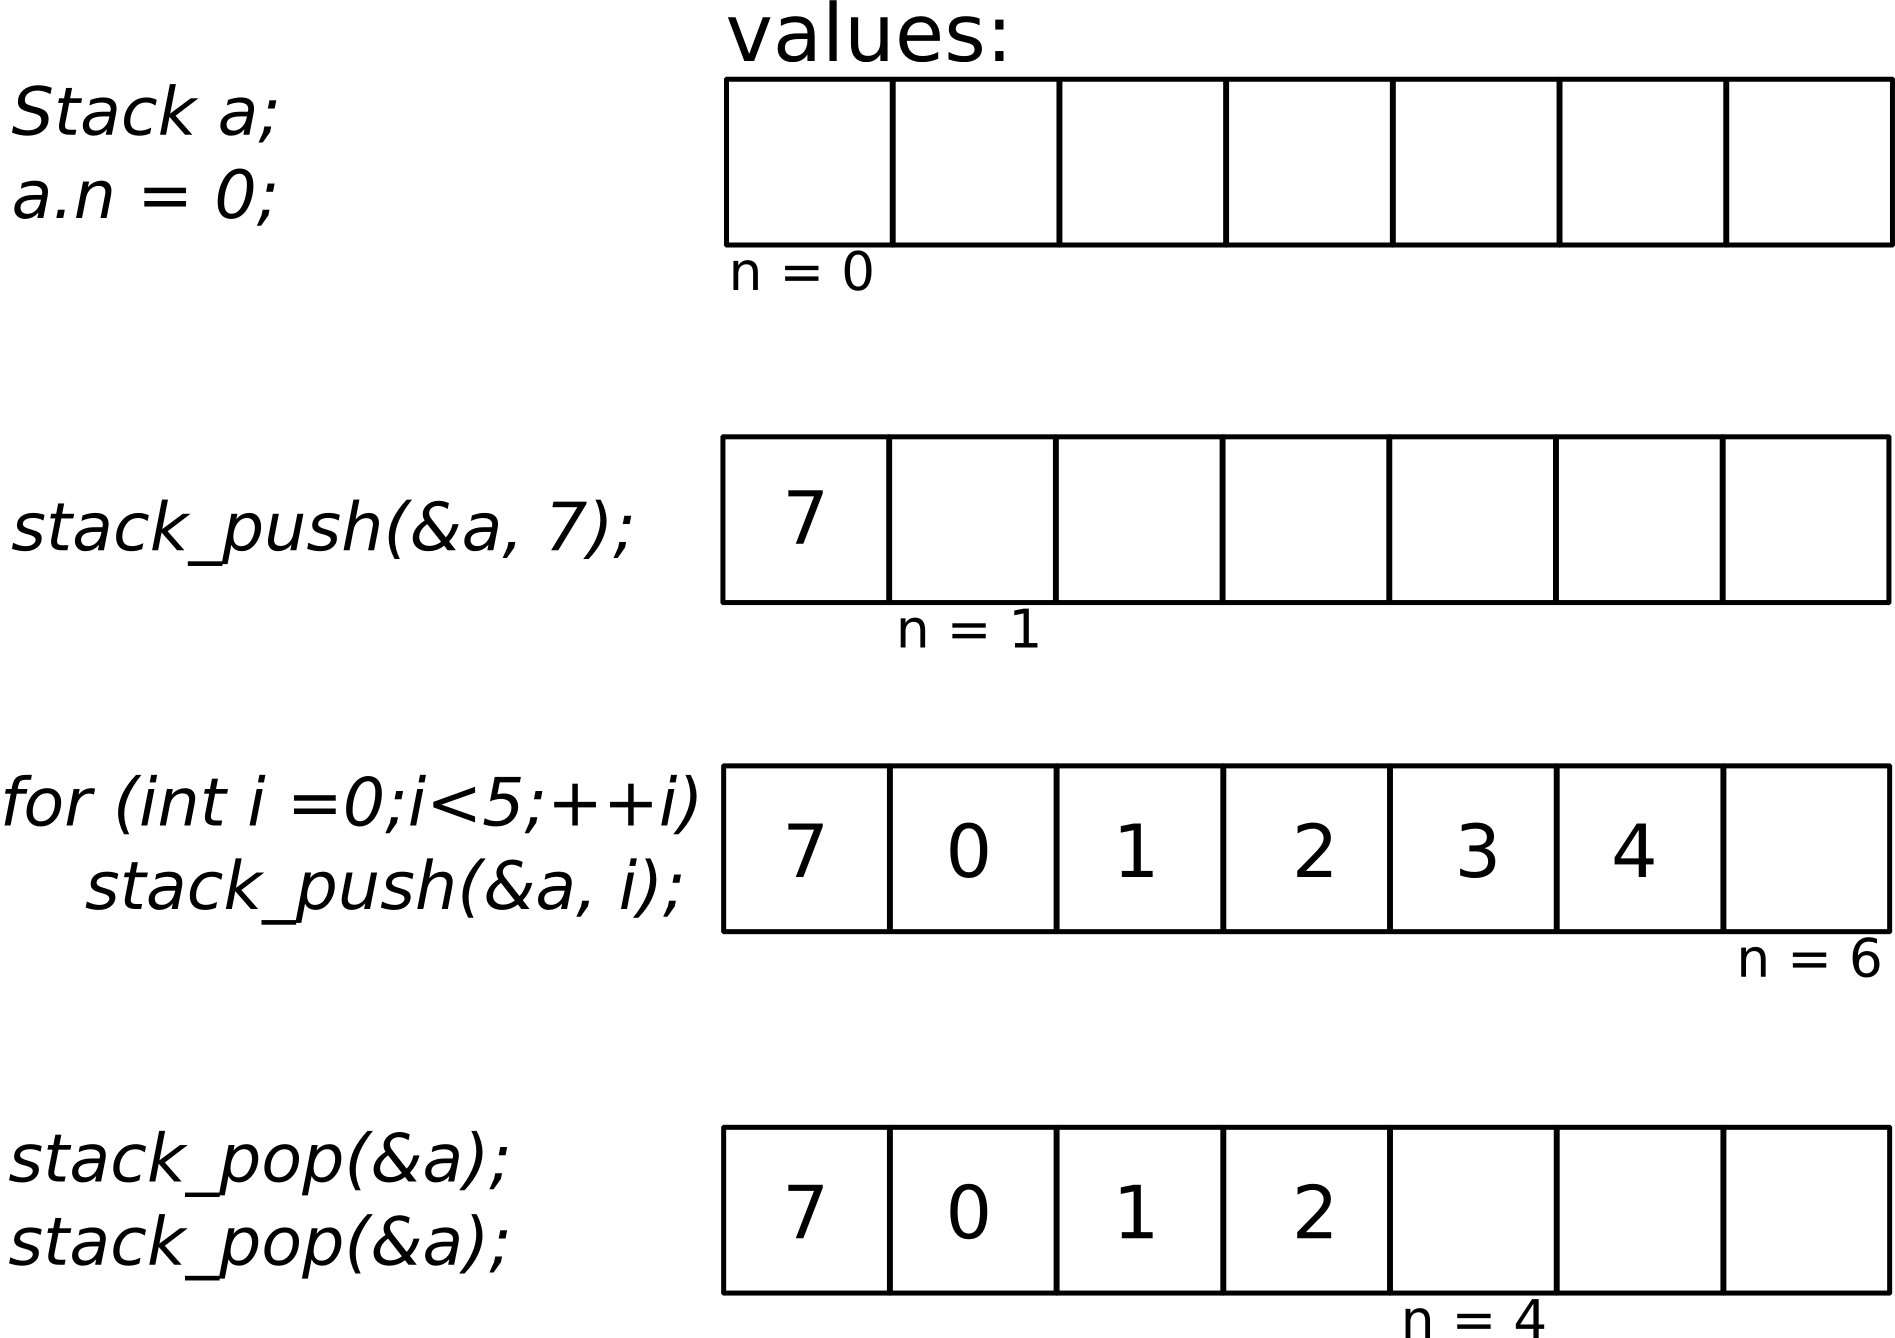
\includegraphics[width=0.95\linewidth]{../images/stack.png}
\end{center}
\end{multicols}
\begin{enumerate}
\item \textbf{Шаблоны 1:} Написать шаблонную функцию \texttt{T max(T x, T y)}, которая возвращает максисум двух переменных. Проверить её на переменных типа int, float, Complex(возможно потребуется написать/придумать оператор сравнения комплексных чисел), строке в стиле C.
\item \textbf{Шаблоны 2::} Написать функцию \texttt{char* max(char* x, char* y)}, для строк в стиле C.
\item \textbf{Шаблоны 3:} Написать шаблонную функцию \texttt{T average(T\& arr[], int count)}, которая возвращает среднее значение массива переменных. Проверить её на переменных типа int, float, Complex.
\item \textbf{Шаблоны 4:} Написать шаблонный класс Array<type> -- динамический массив произвольных элементов. Протестировать его.
\item \textbf{Шаблоны 5*:} Написать шаблонный класс \texttt{template<typename type, int dims> Tensor} -- класс матрицы размерности dims. Напишите функции умножения матрицы на число, вычисление следа(сумма диагональных элементов). Протестируйте этот класс, используйте разные типы и размерности.
\item \textbf{STL vector 1:} Используйте шаблонный класс vector из библиотеки vector. Создайте вектор из чисел 4, 8, 42, 16, 23, 42. Используйте функцию push\_back для добавления чисел в вектор.
\item \textbf{STL vector 2:} Создайте вектор из случайных чисел размера $10^5$, числа от 0 до $10^6$. Для этого целесообразно задать размер вектора в конструкторе или с помощью функции reserve.
\item \textbf{STL vector 3:} Напечатайте все числа в этом векторе, меньшие 1000. Используйте 3 различных обхода вектора.
\item \textbf{STL vector 4:} Напишите функцию \texttt{int is\_exists(const vector<int>\& vec, int x)}, которая будет проверять есть ли в векторе число x.
\item \textbf{STL vector 5:} Отсортируйте вектор с помощью функции sort и напечатайте все числа в этом векторе.
\item \textbf{STL set 1:} Используйте шаблонный класс set из библиотеки set. Создайте вектор из чисел 4, 8, 42, 16, 23, 42. Используйте функцию insert для добавления чисел в множество.
\item \textbf{STL set 2:} Создайте множество и заполните его случайными числами от 0 до $10^6$. 
\item \textbf{STL set 3:} Напечатайте все числа в этом множестве, меньшие 1000. Используйте 2 различных обхода вектора.
\item \textbf{STL set 4:} Проверьте, есть ли в этом множестве число x. Используйте функцию find.
\end{enumerate}

\end{document}